%%
\documentclass[acmlarge, nonacm]{acmart}
\usepackage{graphicx}
\usepackage{hyperref}
%%
%% \BibTeX command to typeset BibTeX logo in the docs
\AtBeginDocument{%
  \providecommand\BibTeX{{%
    Bib\TeX}}}

\begin{document}


\title{Exploring the Impact of an Empathy-Based Sandbox
Approach for Privacy Awareness in Mobile Ecosystems}

\author{Ibrahim Khalilov}
\email{ibrahimk@vt.edu}
% \affiliation{%
%   \institution{Virginia Tech}
%   \state{Virginia}
%   \country{USA}
% }

\maketitle

\section{Introduction}

\subsection{Problem Statement: The Challenge of Mobile Privacy Awareness}

Mobile applications have become an essential part of daily life, providing convenience through services like navigation, social networking, and personalized recommendations. However, these services come at a cost—continuous data collection. Apps frequently request access to GPS location, sensor readings, microphone inputs, browsing activity, and other system data, creating a complex web of data exchange that most users do not fully comprehend. While research has shown that users express concerns about their privacy, their actual behaviors tell a different story, a phenomenon known as the privacy paradox \cite{baruh2017big}. Despite stating that they value privacy, users regularly accept permissions and agree to terms without fully understanding how their data is collected, shared, and utilized \cite{kokolakis2017privacy}.

The issue is exacerbated by the interconnected nature of mobile app permissions. Unlike desktop web tracking, where privacy settings are often confined to cookies or browsing history, mobile applications have deeper access to data that continuously updates in real-time. For instance, enabling GPS for a navigation app might seem straightforward, but in reality, this access can extend to third-party services embedded within the app, such as advertising networks or analytics platforms. Similarly, microphone permissions may allow continuous background audio collection, raising concerns about unintended surveillance \cite{Gao2019}. These permissions often interact in unexpected ways, amplifying privacy risks that users are unaware of.

Compounding this issue, privacy policies remain lengthy, difficult to interpret, and often vague about how collected data is actually used \cite{ObarandOeldorf-Hirsch2020}. Many users accept these terms not because they agree with them but because they have no real choice—denying permissions often means losing access to essential services. Furthermore, even privacy-conscious users struggle to predict the real-world consequences of their privacy choices, leading to uninformed consent.

\subsection{The Role of Sensor Data and Real-Time Privacy Risks}

As mobile applications evolve, real-time sensor data tracking has become increasingly pervasive. Beyond traditional tracking methods like browsing history and IP addresses, modern mobile apps leverage a combination of location, accelerometer, gyroscope, ambient light, battery status, and other sensors to build detailed user profiles. These data points shape personalized user experiences, such as location-based recommendations, targeted advertising, and predictive analytics. While these features enhance usability, they also introduce significant privacy challenges related to transparency and user control \cite{rathi2025predictive}.

Current privacy-enhancing tools—including incognito modes, ad blockers, and permission managers—primarily focus on static privacy protections. For instance, incognito mode prevents browsers from storing history, but it does not stop websites from tracking users via IP addresses, cookies, or fingerprinting techniques. Similarly, ad blockers can block advertisements but do not prevent apps from collecting sensor-based data in real time. These tools, while useful in certain contexts, fail to address the core issue of mobile privacy awareness: helping users understand how their data is continuously being tracked and used. The lack of a risk-free environment where users can test and visualize the impact of their privacy choices makes it difficult for them to make truly informed decisions.

\subsection{Research Questions and Proposed Solution}

To address the gap in privacy awareness, this study introduces an Empathy-Based Privacy Sandbox, a controlled, interactive environment where users can experiment with mobile app permissions, manipulate synthetic data, and observe the consequences of their privacy choices in real time. Existing privacy tools, such as permission managers and system notifications, offer only static, one-time configurations without providing users with an intuitive understanding of how their data influences system behavior over time. In contrast, this sandbox allows users to actively test different privacy settings, modify sensor inputs, and see real-time system adaptations, fostering a more engaging and experiential approach to privacy awareness.

Building on the Empathy-Based Privacy Sandbox framework proposed by \citet{Chaoran2023EmpathySandbox}, this study extends its application beyond web-based environments to mobile ecosystems, where continuous data collection and real-time tracking pose unique privacy challenges. Unlike prior interventions focused on metadata manipulation, this research proposal incorporates sensor data spoofing, advertising identifier manipulation, and behavioral activity simulation—components essential for understanding the dynamic privacy risks of mobile applications. By allowing hands-on experimentation, the sandbox enables users to manipulate the above-mentioned variables to better understand what kind of data can be collected and how it affects system decisions.

This study is guided by the following overarching research question: \textit{How can an interactive, sandbox-based privacy education system enhance mobile users' understanding of data permissions, recognize the extent of their data exposure, and improve informed decision-making?}

To answer this, we further examine:
\begin{itemize}
    \item How do users perceive privacy risks associated with real-time sensor tracking in mobile apps?
    \item How can an empathy-based sandbox improve users’ understanding of how their data footprint influences system behavior?
    \item How does hands-on experimentation with altered mobile data inputs through synthetic personas enhance users’ understanding of privacy risks and influence their decision-making confidence?
\end{itemize}

Through controlled user studies, we aim to evaluate the effectiveness of sandbox-based learning in improving privacy awareness, decision-making, and behavioral shifts. 
% By building upon \citet{Chaoran2023EmpathySandbox}'s methodology, this research offers a more comprehensive framework, integrating key concepts and pioneering a novel approach tailored for mobile systems. It advances HCI scholarship on privacy education, transparency, and user empowerment in digital environments.


% \subsection{Novelty and Contributions}

% While previous research has explored privacy education through just-in-time notifications and text-based policies, these approaches have largely failed to provide an interactive, experiential learning model \cite{feng2021yaodesign}. Recent work by \citet{Chaoran2023EmpathySandbox} introduced an empathy-based privacy sandbox that allows users to explore how manipulated personal information affects system behaviors in web environments. Their study demonstrated that persona-based data experimentation enhances user awareness of privacy risks by enabling controlled manipulation of digital identities. However, their work remains limited to web-based privacy risks, such as cookie tracking, ad personalization, and metadata spoofing, without addressing the more persistent, real-time tracking challenges present in mobile applications.

% This study extends \citet{Chaoran2023EmpathySandbox}'s methodology to mobile ecosystems, adapting and expanding the persona-driven experimentation framework to account for the unique privacy risks of mobile applications, where data collection is continuous, pervasive, and deeply embedded in system functionality. Unlike the web, where tracking largely relies on cookies, browsing history, and explicit user inputs, mobile platforms leverage sensor data, advertising identifiers, and cross-app behavioral patterns to infer user preferences, making privacy risks less transparent and more difficult to control.

% This study makes the following key contributions to HCI and privacy research:
% \begin{itemize}
%     \item 

%     \textbf{Extending Empathy-Based Privacy Awareness Research to Mobile Ecosystems.}
% While prior studies have explored privacy experimentation in web environments, mobile applications present unique challenges due to continuous, real-time data collection, including sensor usage, cross-app tracking, and system-level identifiers. This study expands privacy awareness research to mobile environments, equipping users with new tools to explore how real-time data streams impact app behavior, content personalization, and tracking mechanisms.
    
%     \item \textbf{A Multi-Layered Data Manipulation Framework for Privacy Learning.}
% Unlike previous work that primarily focused on metadata and identity spoofing, our study introduces a broader range of manipulations relevant to mobile privacy. Users can experiment not only with sensor data (e.g., GPS, motion, battery levels) but also advertising identifiers, system-level settings, and behavioral traces—providing a more comprehensive and realistic representation of how their data footprint influences mobile app ecosystems.
% \end{itemize}

% By bridging the gap between abstract privacy policies and real-world data interactions, this study contributes to the broader discourse on usable privacy design in HCI and offers practical design implications for future privacy-enhancing technologies.

\section{Lietrature Review}

\subsection{Privacy Paradox: Why Awareness Alone Fails to Drive Meaningful Privacy Decisions}

Despite increasing public concern over digital privacy, users routinely share personal data without fully understanding its implications. This contradiction, known as the privacy paradox, has been extensively studied \cite{Gerber2018Explaining}. Users often claim to prioritize privacy, yet they regularly accept broad and unrestricted app permissions, demonstrating an inconsistency between attitudes and behaviors \cite{barth2017privacy}, \cite{baruh2017big}.

The privacy paradox arises from several key factors that shape user behavior. One of the primary challenges is cognitive overload, as privacy policies are often excessively long, dense with legal jargon, and difficult to interpret. As a result, many users do not take the time to read or fully understand these policies, leading to uninformed decision-making \cite{Obar2018The}. Another critical factor is the lack of clear mental models regarding how personal data is collected, processed, and shared across different platforms. Without a concrete understanding of these data flows, users struggle to anticipate the real-world consequences of granting permissions, making it difficult to make informed privacy choices \cite{balebako2022nudging}. Additionally, users frequently face convenience versus privacy trade-offs, where denying permissions can result in restricted access to essential apps and services. In many cases, users accept these permissions not because they are comfortable with the privacy implications, but because refusing access would significantly limit their ability to use the app’s core functionalities \cite{Fleischhauer2022Paradox}. These combined factors create an environment where users, despite their stated privacy concerns, routinely engage in behaviors that expose them to greater data collection risks.

While existing privacy awareness efforts focus on educating users via policies, prompts, and notifications, these methods have largely failed to change behavior because they are passive, abstract, and easily ignored \cite{feng2021yaodesign}. This highlights the need for more engaging, interactive approaches that allow users to experience privacy risks in real time.

\subsection{Mobile-Specific Privacy Challenges}
The privacy landscape for mobile applications is distinct from that of traditional web-based environments, as mobile platforms leverage real-time sensor data to track users continuously. Unlike web tracking, which primarily relies on cookies and metadata, mobile applications integrate various built-in sensors—such as GPS, accelerometers, gyroscopes, microphones, ambient light detectors, and others—to monitor user behavior. This real-time data collection poses complex privacy challenges, as it allows for uninterrupted tracking and inference of user activities, often without explicit user awareness \cite{CAHAR}.

Studies have shown that many mobile apps persistently collect location data even when the app is not in use, often sharing it with third-party advertisers and data brokers \cite{bian2021supply}. Similarly, microphone access raises significant privacy concerns, as applications can process ambient audio for targeted advertising or user profiling without clear disclosure \cite{pudasaini2024comprehensive}. Motion sensors and accelerometer data, which were initially designed for fitness tracking and device interactions, have been found to infer users’ routines, detect transportation modes, and even estimate emotional states \cite{niemeijer2023promise}. Furthermore, ambient light sensors and proximity detectors, typically used for screen adjustments, have been exploited for device fingerprinting and covert tracking \cite{berdich2023survey}. Unlike permissions-based access control mechanisms, research indicates that many mobile applications bypass explicit user consent to access sensor data, utilizing indirect inference techniques \cite{aburas2024user}. This makes sensor-based tracking not only a privacy concern but also a security risk, as attackers can manipulate these sensors to extract sensitive behavioral patterns. Given the passive, continuous, and often hidden nature of mobile data collection, traditional privacy tools—such as permission managers and privacy dashboards—fail to provide users with a clear and practical understanding of real-time data exposure.

% To bridge this gap, this study introduces an Empathy-Based Privacy Sandbox, enabling users to experiment with synthetic data in a controlled environment. By allowing users to manipulate their GPS, motion, metadata, and other inputs the sandbox provides firsthand experience of mobile tracking mechanisms, fostering interactive privacy education. This experiential approach aims to shift privacy literacy from passive awareness to active decision-making, equipping users with a deeper understanding of how their sensor data is collected and utilized in mobile ecosystems.

\subsection{Existing Approaches to Privacy Awareness \& Their Limitations}

\begin{table*}[ht]
\centering
\begin{tabular}{|p{3cm}|p{3cm}|p{5cm}|p{4cm}|}
\hline
\textbf{Category} & \textbf{Studies} & \textbf{Study Focus} & \textbf{Limitations} \\ 
\hline
\textbf{Privacy Policies} & \citet{Obar2018The}; \citet{Korunovska2020TheCA}; \citet{burkhardt2023privacy} \citet{stellmacher2022escaping} & Analyzed user engagement with privacy policies, finding that most users ignore them due to complexity. & Does not provide a practical solution to improve privacy comprehension. \\
\hline
\textbf{Just-in-Time Permission Prompts} & \citet{Park2023Understanding}; \citet{Gruber2022Towards}; \citet{bilogrevic2021shhh} & Explored JIT prompts' role in improving privacy awareness but found user fatigue leads to dismissals. & Users ignore frequent prompts, leading to desensitization. \\
\hline
\textbf{Gamified Privacy Education} & \citet{Pahlavanpour2024gamified}; \cite{QUAYYUM2025100826}; \citet{dincelli2020choose}; \citet{stellmacher2022escaping}; \citet{idierukevbe2024bridging} & Investigated game-based learning for privacy awareness, showing increased engagement in controlled studies. & Effectiveness in real-world decision-making remains unclear. \\
\hline
\textbf{Web-Based Privacy Awareness Tools} & \citet{Hasrama2024Exploring}; \citet{bian2021supply} & Developed interactive online tools for privacy education but did not account for mobile-specific tracking. & Lacks applicability to sensor-driven privacy risks. \\
\hline
\textbf{Empathy-Based Sandbox Approaches} & \citet{Chaoran2023EmpathySandbox} & Explored sandbox environments for privacy learning, emphasizing interactive experimentation. & Prior studies focus on metadata manipulation, not real-time sensor tracking. \\
\hline
\textbf{Privacy Management Tools} & \citet{al-muhander2023}; \citet{Stephanidis2025}; \citet{narayanan2024real} & Proposed interactive privacy dashboards and mobile tools for real-time privacy control. & Tools require significant user engagement, which may not be realistic in daily use. \\
\hline
\textbf{Experimental Privacy Education Approaches} & \citet{Fleischhauer2022Paradox}; \citet{aly2024tailoring}; \citet{botturi2023school} & Tested privacy education interventions through controlled lab experiments with mobile users. & Lacks longitudinal studies to measure long-term behavioral impact. \\
\hline
\end{tabular}
\caption{Summary of Prior Research on Privacy Awareness Tools and their limitations in Mobile Ecosystems}
\label{tab:privacy_awareness}
\end{table*}


Several methods have been developed to improve privacy awareness, yet most do not drive significant behavioral change (Table \ref{tab:privacy_awareness}). Privacy policies, despite being legally mandated, are often too lengthy and complex for users to engage with meaningfully, leading to uninformed consent \cite{burkhardt2023privacy}. Just-in-time permission prompts, while intended to enhance user control, frequently result in decision fatigue, causing users to accept permissions without considering the consequences \cite{bilogrevic2021shhh}. Similarly, privacy dashboards, which aggregate data access history, lack real-time tracking insights, limiting their usefulness in preventing unwanted data collection \cite{narayanan2024real}.

Beyond these limitations, ad blockers and tracker prevention tools have proven effective in restricting web-based tracking but are ineffective against sensor-based data collection on mobile devices, which occurs at the system level \cite{bian2021supply}. Gamified privacy education approaches have shown promise in improving user engagement with privacy concepts but often fall short in fostering real-world behavioral changes \cite{idierukevbe2024bridging}. Although sandbox-based privacy education has proven effective in web environments for helping users understand tracking risks \cite{Chaoran2023EmpathySandbox}, its application to mobile ecosystems remains unexplored, despite the unique challenges posed by real-time sensor data collection, as outlined in Table \ref{tab:privacy_awareness}. Most prior sandbox-based interventions have focused on web environments, particularly metadata manipulation like browser attributes and cookie tracking \cite{van2024we}. However, these methods overlook the unique challenges of mobile-specific tracking mechanisms \cite{bella}, underscoring the novelty and significance of this research in advancing the field. Given these shortcomings, there is a clear need for an interactive, real-time learning approach that allows users to actively experiment with mobile privacy settings and understand how their data is being collected and processed.

% \subsection{Empathy-Based Sandboxes in Privacy Research}
% As discussed in Section 2.3, existing privacy awareness tools struggle to provide users with a clear, actionable understanding of mobile tracking mechanisms. In response, sandbox-based interventions have gained traction in privacy research, offering users interactive environments where they can experiment with privacy settings and observe system responses firsthand. Unlike static privacy dashboards or permission managers, which rely on passive information delivery, sandboxes promote experiential learning, allowing users to engage with privacy risks dynamically \cite{Chaoran2023EmpathySandbox}. The studies summarized in Table \ref{tab:privacy_awareness} highlight how sandbox models have been applied in web-based privacy education, yet they have not been adapted to mobile ecosystems, where real-time sensor tracking presents distinct challenges. Most prior sandbox-based interventions have focused on web environments, particularly metadata manipulation like browser attributes and cookie tracking \cite{van2024we}. However, these methods overlook the unique challenges of mobile-specific tracking mechanisms \cite{bella}, underscoring the novelty and significance of this research in advancing the field.

\section{Proposed Research Design and Methodology}
This study employs a lab-based experimental methodology to investigate how interactive, hands-on privacy experimentation in mobile environments influences user understanding of personal data exposure. Building on the empathy-based privacy sandbox framework, this research expands on the methodology previously applied in web environments \cite{Chaoran2023EmpathySandbox} to mobile applications, incorporating real-time data manipulations that are uniquely tied to mobile ecosystems, as illustrated in Figure \ref{fig:methodology}. The study design consists of a controlled experimental setup where participants will engage with the \textit{Empathy-Based Privacy Sandbox for Mobile}, allowing them to explore the consequences of privacy decisions in a risk-free setting. The methodological framework is structured around a three-phase approach: (1) an introduction and familiarization phase, (2) an interactive experimental phase, and (3) a post-experiment reflection phase.

\begin{figure}[htbp]
    \centering
    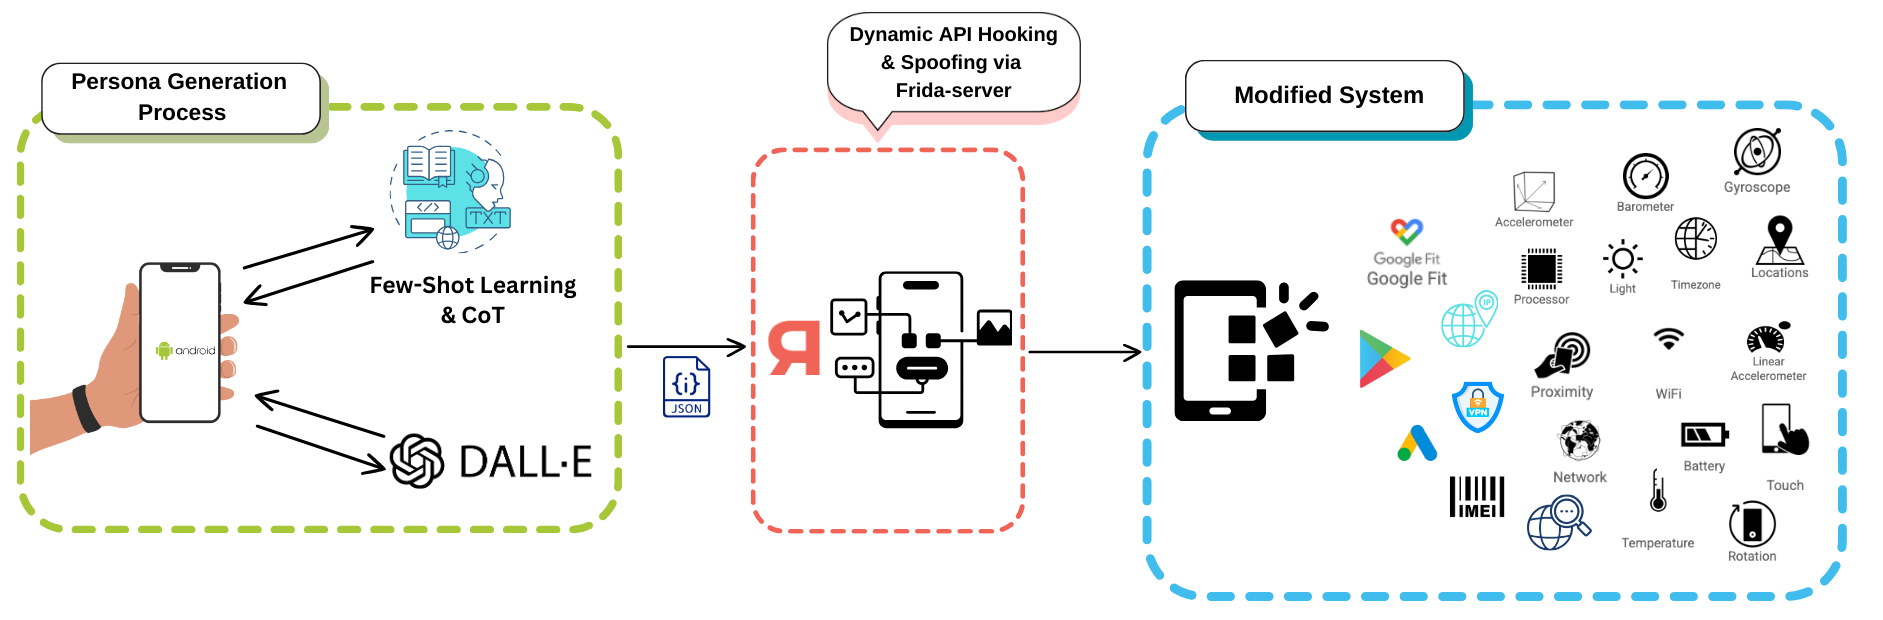
\includegraphics[width=\textwidth]{figure-2-methodology.png} 
    \caption{Pipeline for Persona Generation and Real-Time Data Spoofing}
    \label{fig:methodology}
\end{figure}

\subsection{Empathy-Based Privacy Sandbox for Mobile}

The \textit{Empathy-Based Privacy Sandbox for Mobile} serves as the experimental testbed for this study, providing participants with an interactive platform where they can actively modify privacy settings, alter real-time data streams, and observe system responses (Figure \ref{fig:methodology}). Unlike traditional privacy education tools that rely on passive explanations or abstract warnings, this sandbox enables users to directly manipulate data attributes such as mobile permissions, sensor readings, advertising identifiers, and behavioral activity patterns. By engaging with the sandbox, participants can witness in real time how mobile applications react to different privacy configurations, fostering a deeper, experiential understanding of how their data is collected, shared, and utilized.

The sandbox environment supports both guided and self-directed privacy exploration. Participants will initially follow structured privacy manipulation tasks designed to highlight key areas of mobile data tracking, such as location tracking, motion-based personalization, and advertising personalization. Following this, they will transition to an open-ended phase where they can explore data modifications independently. A real-time feedback system within the sandbox provides users with immediate insights into how their changes impact app behavior, allowing them to make connections between privacy settings and personalization mechanisms.
\subsection{Persona Generation and Spoofing}

A persona is a constructed identity that represents a typical user, complete with demographic details, behavioral patterns, and digital interactions. In privacy research, personas serve as a controlled way to explore data collection and system responses without exposing real user information \cite{persona}, \cite{Chaoran2023EmpathySandbox}. By simulating real-world behaviors—such as browsing habits, app usage, and sensor interactions—personas allow participants to experience privacy risks firsthand. This immersive approach not only enhances understanding but also fosters empathy, as users see how different privacy choices shape their digital experiences.

The process of persona generation and data spoofing in this study follows a structured pipeline that integrates \textit{few-shot learning}, \textit{chain-of-thought reasoning}, and \textit{real-time system spoofing} to create synthetic mobile personas (Figure \ref{fig:methodology}). These personas mimic real user behaviors, allowing participants to explore privacy risks in a controlled, interactive environment without exposing their actual data.

\textbf{Persona initialization.} The process begins with persona initialization, where users provide a brief textual description to guide the creation of a synthetic identity. This input may include factors such as occupation, lifestyle, and typical mobile habits. To generate a coherent and contextually relevant persona, we apply few-shot learning, feeding a pre-trained language model with structured examples of realistic mobile users. This helps the model infer missing details such as socioeconomic background, device preferences, and common app usage patterns.

To ensure that each persona behaves in a way that aligns with real-world usage patterns, we apply context-aware refinement. This means that generated attributes—such as location history, browsing behavior, and notification interactions—are dynamically adjusted based on previously generated data points. For example, if a persona frequently uses a fitness tracking app, their accelerometer and step count data will reflect regular activity patterns rather than random fluctuations. This step ensures that browsing history, location check-ins, and app engagement patterns evolve in a way that mirrors actual user behavior rather than isolated, randomly generated events.

\textbf{Timeline of interaction. }Following this, we use chain-of-thought reasoning to generate a timeline of interactions. Instead of creating standalone data points, the model constructs a logical sequence of actions, simulating how a persona might use their mobile device throughout the day. For example, if the persona starts their day checking a news app, they might later visit a social media app where similar news stories appear due to targeted recommendations. If they use a fitness app in the morning, their persona might later check their hydration or step count progress via a health-tracking application. By structuring events as a logical sequence, we enhance the realism of the synthetic behavior.

To make the persona visually tangible, we generate a synthetic profile image. This involves structuring the persona’s demographic attributes into a detailed prompt, which is then processed by a generative model such as DALLE \cite{dalle} or Stable Diffusion \cite{stablediffusion}. The resulting image is refined to ensure alignment with the persona’s generated characteristics, improving realism and relatability.

\textbf{System Spoofing.} Once the persona is fully formed, we integrate it into the mobile system by replacing key identifiers and injecting real-time synthetic data. This is achieved using a Frida-server running continuously on the Android device, which allows dynamic hooking into system-level APIs \cite{frida}. Through custom Frida scripts, we intercept and modify data at the system level, ensuring that any request for sensor data—such as GPS location, accelerometer readings, gyroscope outputs, battery status, or ambient light levels—returns synthetic values aligned with the persona's behavioral profile. This ensures that applications interact with the synthetic persona rather than the real user.

To prevent cross-app tracking, we integrate Google Ad ID spoofing, session-based context switching, and device fingerprint mimicking, ensuring that applications cannot persistently track a persona across different persona sessions. Each time a user selects a new persona, all identifiers are reset, preventing residual tracking from previous interactions. By dynamically modifying the Google Ad ID, we disrupt ad targeting and recommendation systems, ensuring that each persona is treated as a distinct user. Session-based context switching further reinforces identity separation by altering IP addresses, MAC addresses, and WiFi SSIDs, with a VPN-based module routing traffic through geographically relevant proxies to match the persona’s designated behavior. Additionally, we mitigate device fingerprinting, which relies on hardware and software traits for tracking, by using Frida hooks to modify API responses and randomize system parameters. This ensures that each persona session presents a unique device configuration, preventing persistent tracking across personas within the lab study.

\textbf{Experimental set-up.} During the experiment, the persona engages with mobile applications as a real user would. If a weather app requests temperature and location data, the sandbox provides geolocation and weather conditions consistent with the persona’s profile. If a fitness app queries motion sensors, it receives activity patterns that reflect the persona’s simulated routine, such as walking or running data. If an e-commerce app requests browsing history for personalized recommendations, the sandbox provides a synthetic search and purchase history aligned with the persona’s shopping habits. This hands-on manipulation allows participants to observe how mobile applications process personal data and adjust their responses based on user attributes.

By combining few-shot learning, chain-of-thought reasoning, and real-time system spoofing, this methodology creates a highly immersive and technically robust empathy-based sandbox tailored for mobile privacy research. This approach enables users to gain a deeper understanding of how their data is collected and utilized in real time, reinforcing the effectiveness of interactive privacy education in mobile environments. Additionally, by immersing users in the experiences of their generated personas, this method fosters empathy, allowing them to see firsthand how different privacy choices impact digital interactions and data exposure \cite{Chaoran2023EmpathySandbox}. This perspective shift enhances user engagement, making privacy risks more tangible and personally relevant.


\subsection{Study Procedure}

The study consists of three structured phases: (1) a pre-experiment familiarization phase, (2) an interactive experimental phase, and (3) a post-experiment reflection phase.

In the pre-experiment phase, participants will complete a questionnaire assessing their existing knowledge of mobile privacy risks, familiarity with mobile data collection practices, and general privacy attitudes. This baseline data will serve as a reference point for evaluating potential changes in user awareness and understanding throughout the study. Participants will then receive a brief introduction to mobile privacy issues, the function of the sandbox, and how they will interact with the system.

During the experimental phase, participants will engage in structured interactions with the sandbox. In the guided privacy manipulation phase, they will follow a set of pre-defined tasks designed to help them explore key aspects of mobile data collection. Tasks will include modifying permissions, spoofing sensor inputs, adjusting advertising identifiers, and restricting app access to personal data. A real-time feedback system will display how these changes impact app behavior, reinforcing an experiential learning model that fosters privacy awareness.

Following the guided phase, participants will enter a self-directed exploration phase, where they will have full control over privacy modifications. This phase will allow researchers to observe how users engage with the sandbox when given autonomy, providing insights into their decision-making processes and perceptions of privacy risks.

In the post-experiment reflection phase, participants will complete a follow-up questionnaire assessing how their perceptions of mobile privacy have changed. Additionally, semi-structured interviews will be conducted, allowing participants to discuss their experiences, key takeaways, and reflections on their understanding of mobile privacy risks. This qualitative data will provide a deeper understanding of how experiential learning influences privacy awareness and decision-making confidence.

% By systematically evaluating user interactions, learning patterns, and reflections, this study aims to assess whether sandbox-based privacy learning remains an effective tool in mobile ecosystems. The findings will offer insights into the usability, effectiveness, and potential design improvements for future privacy-enhancing technologies.


\subsection{Study Design: Data Collection and Analysis.}

The study follows a controlled experimental design conducted in a laboratory environment, where participants will interact with the sandbox under varying privacy manipulation conditions. The goal of this setup is to assess whether hands-on interaction with privacy manipulations improves user understanding of mobile data exposure. A total of 10 to 15 participants will be recruited, ensuring diversity in terms of privacy attitudes, technical proficiency, and behavioral patterns.

Participants will be assigned to different experimental conditions, each designed to test distinct aspects of privacy decision-making. In the baseline condition, participants will interact with mobile applications using default privacy settings, establishing an initial reference point for how users typically experience mobile data collection. In the guided privacy manipulation condition, they will be instructed to systematically alter privacy settings, modifying sensor inputs, adjusting advertising identifiers, and restricting permissions to observe how these changes influence app behavior. The final condition, a self-directed exploration phase, will allow participants to experiment freely with privacy settings, enabling researchers to examine how autonomy in privacy decision-making shapes user perceptions and actions.

User interactions will be logged and analyzed, tracking which privacy modifications participants engage with most frequently, how they interpret system responses, and whether they develop a clearer understanding of their personal data exposure. This empirical evaluation of user-driven privacy manipulations will provide insights into whether interactive engagement fosters more informed decision-making compared to conventional privacy education methods.

% The goal of this setup is to assess whether hands-on interaction with privacy manipulations improves user understanding of mobile data exposure. This study evaluates if the sandbox approach remains effective in mobile environments by allowing users to modify permissions, sensor inputs, and identifiers, providing real-time feedback on how their data is processed and influencing privacy decisions.


\section{Planned Evaluation and Expected Outcomes}
The evaluation of this study will focus on assessing the effectiveness of the \textit{Empathy-Based Privacy Sandbox for Mobile} in enhancing users' understanding of mobile data exposure. By observing user interactions, behavioral shifts, and reflections within the experimental environment, we aim to gain insights into how experiential privacy education influences decision-making and awareness.

\subsection{Expected Impact on Privacy Awareness}

The Empathy-Based Privacy Sandbox is designed to foster a deeper understanding of mobile data flows by allowing users to manipulate and observe real-time system responses. Unlike static privacy education methods, this interactive approach is expected to provide users with firsthand experience of how their data is collected, processed, and repurposed by mobile applications. We anticipate that users will develop stronger mental models of mobile privacy risks, enabling them to make more informed decisions when managing app permissions and data-sharing settings.

\subsection{Anticipated User Reactions}
Participants will likely exhibit a range of emotional and cognitive responses as they engage with the sandbox environment. Some users may experience surprise or concern upon realizing the extent of their data exposure, while others may express frustration over the lack of transparency in mobile privacy settings. Additionally, users who previously assumed their data was secure may undergo a shift in perception as they witness how easily system behaviors can be influenced by modifying inputs such as sensor readings and advertising identifiers. These reactions will provide valuable qualitative insights into the psychological dimensions of privacy awareness.

\subsection{Behavioral Adjustments Post-Experiment}
A key outcome of this study is to assess whether exposure to the Empathy-Based Privacy Sandbox leads to long-term changes in privacy-related behaviors. We expect that users who engage with the sandbox will become more proactive in managing app permissions, adjusting privacy settings, and questioning data collection practices. These behavioral shifts will be measured through post-experiment debriefs, where participants will reflect on their learning experience and indicate any planned changes to their mobile privacy habits. If the sandbox proves effective, we anticipate that users will express increased confidence in navigating privacy settings and demonstrate a more critical approach to granting app permissions.

% \subsection{Comparison to Traditional Privacy Tools}
% Traditional privacy tools, such as permission managers and privacy dashboards, provide users with options to limit data collection but fail to convey the full scope of real-time data exposure. Unlike these static tools, the Empathy-Based Privacy Sandbox offers an immersive, hands-on experience that actively engages users in experimenting with their own data. This study aims to highlight the limitations of conventional privacy education approaches and demonstrate the added value of interactive, real-time experimentation in fostering privacy awareness. While traditional tools are designed for direct data control, they often lack the educational and experiential components necessary for users to develop a deeper understanding of privacy risks. By positioning the sandbox as a complement to existing privacy tools, this study contributes to the broader discourse on designing more effective and user-centered privacy interventions.

\section{Discussion and Broader Implications}

This study contributes to ongoing discussions in Human-Computer Interaction (HCI) and Privacy Research by exploring how an Empathy-Based Privacy Sandbox can enhance user understanding of mobile data exposure. By offering an interactive and experiential approach to privacy education, we aim to bridge the gap between privacy attitudes and actual behaviors, equipping users with the knowledge and confidence to make informed data-sharing decisions.

\subsection{Contributions to HCI and Privacy Research}

This research extends the Empathy-Based Privacy Sandbox framework into mobile environments, addressing a critical gap in privacy education for sensor-driven ecosystems. While prior studies have primarily focused on web-based interventions, our study introduces a hands-on, mobile-first approach that allows users to experiment with real-time data streams, including sensor inputs, advertising identifiers, and system-level settings. This work advances HCI scholarship by emphasizing the role of interactive learning environments in fostering privacy literacy and decision-making confidence among mobile users.

Furthermore, this study validates the effectiveness of an empathy-based sandbox approach in mobile ecosystems, reinforcing the idea that direct engagement with privacy risks can lead to stronger mental models of data exposure. By demonstrating how user-centered, experiential learning can drive behavioral shifts, our research informs future design frameworks for privacy-enhancing technologies in mobile computing.

\subsection{Implications for Mobile App Design and Policy}
The findings of this study have practical implications for mobile app developers, UI/UX designers, and policymakers. Current privacy tools—such as privacy dashboards and permission managers—provide only static, reactive controls, often leaving users unaware of how their data is continuously collected and utilized. This study highlights the need for more interactive, real-time feedback mechanisms that allow users to explore privacy settings dynamically.

For mobile app developers, integrating sandbox-like privacy simulations could improve user trust and compliance with transparency regulations. By offering in-app privacy experimentation features, developers can empower users to understand the effects of different privacy configurations without the fear of permanent consequences.

For policymakers and regulatory bodies, this research supports the argument for enhanced user control mechanisms that go beyond simplistic opt-in/opt-out models. The European Union’s GDPR and the California Consumer Privacy Act (CCPA) have emphasized the need for transparency, but current implementations often fail to communicate privacy risks effectively. By demonstrating the educational value of an interactive sandbox approach, this study provides empirical evidence for policy recommendations aimed at improving privacy education and user agency.

\subsection{Limitations and Future Directions} 

While this study advances privacy education in mobile ecosystems, it has certain limitations that also present opportunities for future research. One major constraint is the challenge of real-time data manipulation within mobile environments. Unlike web-based privacy interventions, mobile applications operate in tightly controlled, sandboxed systems that restrict cross-app interactions and data modifications. Our approach mitigates some of these limitations through app-specific interventions, but broader system-level strategies may be necessary to fully address privacy risks that span multiple applications and services.  

Another limitation is the controlled nature of our study. Conducting experiments in a lab setting allows for precise measurement of user interactions, but it does not fully capture how users make privacy decisions in everyday contexts. Future research should explore longitudinal studies that assess whether hands-on privacy experimentation leads to sustained improvements in privacy literacy and decision-making confidence over time. Additionally, deploying sandbox-based privacy tools in real-world scenarios could provide deeper insights into how users engage with these interventions outside of a structured environment.  

This study also focuses exclusively on Android devices, utilizing system-level API hooking and sensor spoofing to simulate privacy manipulations. While Android allows for significant modifications at the system level, Apple’s stricter security policies and the constraints of its App Tracking Transparency (ATT) framework \cite{apple_att} limit similar interventions on iOS. Expanding this research to include iOS and other operating systems would provide a more comprehensive understanding of platform-specific privacy challenges and help develop cross-platform privacy solutions.  

Future work should also consider integrating adaptive learning mechanisms into privacy sandboxes. Personalized feedback and dynamic privacy simulations could improve engagement and usability across diverse user groups by tailoring experiences to individual knowledge levels and concerns. Moreover, collaborating with industry stakeholders—such as app developers, privacy advocates, and regulatory bodies—could enable the integration of sandbox-based privacy interventions into commercial applications. This could provide valuable insights into their effectiveness in influencing user behavior, enhancing trust, and ensuring compliance with evolving privacy regulations.  

By addressing these limitations and expanding the research across different platforms, environments, and user demographics, future studies can refine and validate sandbox-based approaches as a central tool for privacy education and user empowerment in mobile ecosystems.

% \subsection{Challenges and Potential Limitations}

% Despite its contributions, this study faces several challenges and limitations. One key challenge is the complexity of real-time data manipulation on mobile devices. Unlike web-based privacy interventions, mobile applications operate within sandboxed environments, limiting cross-app interactions and restricting certain data manipulations. While our study circumvents some of these limitations by focusing on app-specific behaviors, future work may need to explore broader system-level interventions.

% Another limitation is the controlled nature of the study. Because this research is conducted in a lab environment, user behaviors may not fully reflect real-world interactions with privacy settings. While our study provides valuable insights into privacy awareness, additional longitudinal studies will be necessary to assess the long-term impact of sandbox-based privacy education on user decision-making. 

% Moreover, this study was conducted exclusively on Android devices, leveraging system-level API hooking to manipulate sensor data and user identifiers. While Android provides greater flexibility for modifying system behaviors, the same level of intervention may not be feasible on iOS, where Apple enforces stricter security and privacy controls. As a result, the findings may not fully generalize to iOS ecosystems.

% Furthermore, the effectiveness of this approach may vary across different user demographics. Prior research suggests that privacy literacy, technical expertise, and cultural differences all influence privacy-related behaviors. Future research should explore how different user groups respond to sandbox-based privacy interventions and whether customization or adaptive guidance could enhance usability across diverse populations.



% \subsection{Future Research Directions}

% This study lays the groundwork for several future research directions in HCI and privacy research. One avenue is the integration of adaptive learning models into privacy sandboxes. By leveraging personalized feedback mechanisms, future versions of the sandbox could dynamically adjust privacy simulations based on user expertise and privacy concerns.

% Additionally, expanding the scope of the study to real-world deployment scenarios could provide valuable insights into long-term behavioral changes. While this research focuses on immediate user reactions, future work should examine whether hands-on privacy experimentation leads to sustained improvements in privacy literacy and decision-making confidence over time.

% Furthermore, future research should explore how similar privacy-enhancing techniques could be adapted for iOS, particularly in light of Apple's App Tracking Transparency (ATT) framework \cite{apple_att} and its restrictions on background data access. Investigating how cross-platform tracking mechanisms operate between Android and iOS users could provide deeper insights into privacy risks in mixed-device environments.

% Lastly, future research could explore collaborations with industry stakeholders, including app developers, privacy advocates, and regulatory bodies, to integrate sandbox-based privacy interventions into commercial applications. By partnering with technology companies, future studies could assess how such interventions impact user trust, engagement, and compliance with evolving privacy regulations.

% By addressing these challenges and extending this research to new contexts, future work can further refine and validate sandbox-based approaches as a core component of privacy education and user empowerment in mobile ecosystems.

\section{Conclusion}

The proposed research introduces an Empathy-Based Privacy Sandbox for mobile ecosystems, aiming to address the challenges of real-time data collection and tracking. Unlike traditional privacy tools that rely on static settings, this approach enables users to dynamically manipulate their data footprint and observe system responses, fostering privacy literacy and informed decision-making. By extending empathy-driven privacy interventions to mobile environments, this study explores the effectiveness of interactive, hands-on learning in bridging the gap between privacy attitudes and behaviors. While designed as a controlled lab study, this research lays the groundwork for evaluating mobile privacy risks and informing future privacy-enhancing technologies. Limitations, such as the focus on Android devices, highlight opportunities for expanding the study to cross-platform privacy dynamics and assessing long-term behavioral impacts. As mobile privacy concerns continue to grow, this proposal underscores the need for experiential privacy education that empowers users and promotes more transparent, user-centric digital ecosystems.

% This study introduces an Empathy-Based Privacy Sandbox for mobile ecosystems, extending prior work on privacy awareness to address the unique challenges of mobile data collection. Unlike traditional privacy tools, which provide static and often abstract privacy controls, our sandbox allows users to actively manipulate their data footprint and observe system responses in real time. By enabling hands-on experimentation with mobile-specific data streams, such as sensor inputs, advertising identifiers, and system-level interactions, this approach enhances privacy literacy and decision-making confidence among users.

% The primary contribution of this study is the development of an interactive, human-centered learning framework that empowers users to better understand how their personal data is collected, processed, and leveraged by mobile applications. By offering a controlled, risk-free environment, this research bridges the gap between privacy attitudes and behaviors, demonstrating that experiential learning can be a powerful tool for enhancing user agency in privacy management.

% Furthermore, our study contributes to HCI and privacy research by validating the effectiveness of sandbox-based privacy education in a mobile setting. While previous research has established the benefits of empathy-driven privacy interventions in web environments, this study extends these findings by exploring their applicability to mobile ecosystems with a new methodology, where continuous, real-time tracking mechanisms present new and underexplored privacy risks. The study also informs future design considerations for mobile app developers, policymakers, and privacy advocates, highlighting the need for interactive, transparent, and user-controllable privacy mechanisms beyond simple opt-in/opt-out models.

% Despite its contributions, this research is not without limitations. The controlled lab environment of our study, while valuable for evaluating initial user reactions, may not fully reflect long-term privacy behaviors in real-world settings. Future work should explore longitudinal studies to assess how sustained engagement with privacy sandboxes influences user decision-making over time. Additionally, further refinement of interactive privacy tools—potentially incorporating adaptive learning models—could enhance personalization and usability across diverse user groups. Moreover, our implementation is currently limited to Android devices, which presents both a constraint and an opportunity. While this limitation means that our findings may not fully capture privacy challenges and system behaviors on other platforms, such as iOS, it also opens the door for future research to explore cross-platform privacy dynamics. Broadening the scope to multiple operating systems could provide deeper insights into mobile privacy risks and inform more universally applicable mitigation strategies.

% As mobile privacy concerns continue to grow, empowering users with experiential learning tools becomes increasingly critical. This study lays the groundwork for future advancements in privacy education, reinforcing the idea that hands-on engagement with privacy settings is essential for fostering meaningful behavioral change. By expanding the scope of privacy-enhancing technologies, this research contributes to the broader discourse on usable privacy design and provides actionable insights for building more transparent, user-centric mobile applications.


\bibliographystyle{ACM-Reference-Format}
\bibliography{sample-base}

\end{document}
\endinput
%%
%% End of file `sample-acmlarge.tex'.
